\documentclass{beamer}
\usepackage[utf8]{inputenc}

\usetheme{Madrid}
\usecolortheme{default}
\usepackage{amsmath}
\usepackage{amssymb,amsfonts,amsthm}
\usepackage{txfonts}
\usepackage{tkz-euclide}
\usepackage{listings}
\usepackage{adjustbox}
\usepackage{array}
\usepackage{tabularx}
\usepackage{gvv}
\usepackage{lmodern}
\usepackage{circuitikz}
\usepackage{tikz}
\usepackage{graphicx}
\usepackage{float}

\setbeamertemplate{page number in head/foot}[totalframenumber]

\usepackage{tcolorbox}
\tcbuselibrary{minted,breakable,xparse,skins}

\definecolor{bg}{gray}{0.95}
\DeclareTCBListing{mintedbox}{O{}m!O{}}{%
  breakable=true,
  listing engine=minted,
  listing only,
  minted language=#2,
  minted style=default,
  minted options={%
    linenos,
    gobble=0,
    breaklines=true,
    breakafter=,,,
    fontsize=\small,
    numbersep=8pt,
    #1},
  boxsep=0pt,
  left skip=0pt,
  right skip=0pt,
  left=25pt,
  right=0pt,
  top=3pt,
  bottom=3pt,
  arc=5pt,
  leftrule=0pt,
  rightrule=0pt,
  bottomrule=2pt,
  toprule=2pt,
  colback=bg,
  colframe=orange!70,
  enhanced,
  overlay={%
    \begin{tcbclipinterior}
    \fill[orange!20!white] (frame.south west) rectangle ([xshift=20pt]frame.north west);
    \end{tcbclipinterior}},
  #3,
}
\lstset{
    language=C,
    basicstyle=\ttfamily\small,
    keywordstyle=\color{blue},
    stringstyle=\color{orange},
    commentstyle=\color{green!60!black},
    numbers=left,
    numberstyle=\tiny\color{gray},
    breaklines=true,
    showstringspaces=false,
}

\title{1.9.14}
\date{29th August, 2025}
\author{AI25btech11014-Suhas}
\graphicspath{{./figs/}}

\begin{document}

\frame{\titlepage}

\begin{frame}{Question}
Show that the points  
$\vec{A} = \myvec{2\\3\\-4}$,  
$\vec{B} = \myvec{1\\-2\\3}$,  
$\vec{C} = \myvec{3\\8\\-11}$  
are collinear.
\end{frame}

\begin{frame}{Theoretical Solution}
Compute direction vectors:  
\begin{align}
\vec{B} - \vec{A} &= \myvec{1\\-2\\3} - \myvec{2\\3\\-4} = \myvec{-1\\-5\\7} \\
\vec{C} - \vec{A} &= \myvec{3\\8\\-11} - \myvec{2\\3\\-4} = \myvec{1\\5\\-7}
\end{align}
\end{frame}

\begin{frame}{Matrix Construction}
Form matrix $M$ with direction vectors as rows:
\begin{align}
M = \myvec{-1 & -5 & 7\\1 & 5 & -7}
\end{align}
We will perform row operations to determine the rank.
\end{frame}

\begin{frame}{Row Operations}
Swap rows:
\begin{align}
\myvec{1 & 5 & -7\\-1 & -5 & 7}
\end{align}
Apply $R_2 \rightarrow R_2 + R_1$:
\begin{align}
\myvec{1 & 5 & -7\\0 & 0 & 0}
\end{align}
\end{frame}

\begin{frame}{Conclusion}
Only one non-zero row remains:
\begin{align}
\text{Rank}(M) = 1
\end{align}
Therefore, the vectors are linearly dependent.  
\[
\textbf{Hence, the points are collinear.}
\]
\end{frame}

\begin{frame}[fragile]
\frametitle{C Code - Direct Solve}
\begin{lstlisting}
#include <stdio.h>

int main() {
    float M[2][3] = {
        {-1, -5, 7},
        {1, 5, -7}
    };

    for (int i = 0; i < 3; i++)
        M[1][i] += M[0][i];

    if (M[1][0] == 0 && M[1][1] == 0 && M[1][2] == 0)
        printf("Points are collinear\n");
    else
        printf("Points are not collinear\n");
}
\end{lstlisting}
\end{frame}

\begin{frame}[fragile]
\frametitle{C Code - Function for .so}
\begin{lstlisting}
#include <stdio.h>

int check_collinear() {
    float M[2][3] = {
        {-1, -5, 7},
        {1, 5, -7}
    };

    for (int i = 0; i < 3; i++)
        M[1][i] += M[0][i];

    return (M[1][0] == 0 && M[1][1] == 0 && M[1][2] == 0);
}
\end{lstlisting}
\end{frame}

\begin{frame}[fragile]
\frametitle{Python Code - Shared Output}
\begin{lstlisting}
import ctypes

lib = ctypes.CDLL("./libcollinear.so")
lib.check_collinear.restype = ctypes.c_int

result = lib.check_collinear()
if result == 1:
    print("Points A, B, C are collinear")
else:
    print("Points are not collinear")
\end{lstlisting}
\end{frame}

\begin{frame}{Plot}
\begin{figure}
    \centering
    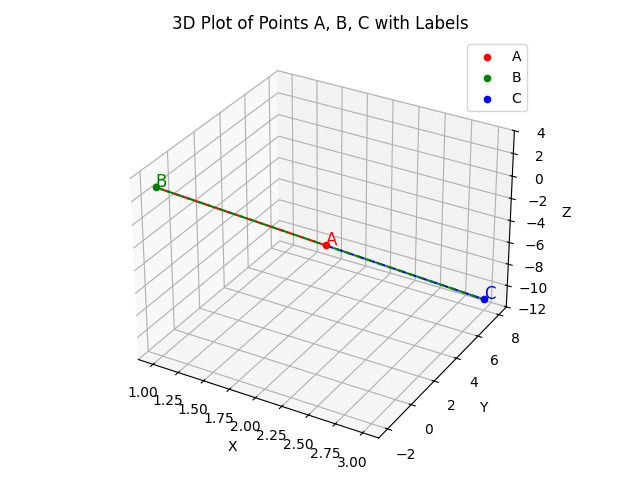
\includegraphics[width=0.9\textwidth]{figs/fig1.png}
    \caption{3D Visualization of Points A, B, C}
\end{figure}
\end{frame}

\end{document}